\documentclass[12pt,a4paper]{article}
\usepackage{amsmath}	
\usepackage{graphicx}			
\begin{document}
\title{Optimal state observer for linear systems Lecture Notes} 
\author {Fadi Younes}
\maketitle
\newpage
\section*{Overview}
A state observer provides internal state estimation by measuring the Input and output of real given system. The system states are compulsory to solve control engineering problems like state feedback stabilization of system. It is used to reconstruct the system state from output measurement only if system is observable. 
\section*{Linear time invariant (LTI) system}
It is assumed that the state of linear time invariant (LTI) physical discrete-time system satisfies, \cite{khalil2002nonlinear}\\
\begin{equation}
x(k+1) = Ax(k) + Bu(k)
\end{equation}
\begin{equation}
y(k) = Cx(k) + Du(k)
\end{equation}\\
Where plant state is represented by x (k) at time ‘k’, u (k) is an input and y (k) is the output of the system. Merely such equations defines that current inputs and current states is solely responsible to determine the future states and current output of plant. However same equations can be used to analyze the continuous time linear invariant system with continuous time step. System observation can be determined by observable matrix and if it is observable then y (k) can be utilized to get states of the system.
\section*{Observer design}
The state observer model of given system is derived from equation 1 and 2. The successive calculated values of input and output of plant is ensured by adding additional term in above equations, so that state converges to plant. The state observer called Luenberger observer, constructed by adding the following term in above equation no 1 \cite{bernat2015multi}.\\
\begin{align*}
L[y(k)-\hat{y(k)}]
\end{align*}
Where observer output is subtracted from plant output and then multiplied by ‘L’ matrix. Then it summarized as,
\begin{equation}
\hat{x(k+1)} = A\hat{x(k)} + L[y(k)-\hat{y(k)}]+ Bu(k)
\end{equation}
\begin{equation}
\hat{y(k)} = C\hat{x(k)} + Du(k)
\end{equation}
The designed observer is stable if and only if error e (k) approaches to zero when discrete time step ‘k’ leads to infinity.
\begin{equation}
e(k)= \hat{x(k)}-x(k)
\end{equation}
\section*{Asymptotic stability}
The Luenberger observer satisfies if and only if error e (k+1) approaches to zero when discrete time step ‘k’ leads to infinity  \cite{pasand2019luenberger}.\\
\begin{equation}
e(k+1)= (A-LC)e(k)
\end{equation}
The asymptotic stability of Luenberger observer is associated with Eigenvalue values of (A-LC) matrix. If eigenvalues lies in inside the unit circle then it is asymptotic stable.
\section*{Optimal minimal order state observer}
The reduced order or minimal order state observer are called optimal observer that gives us least mean square estimation error in all 'n-m' dimensional filter. where n represent the system state dimension to be estimated and 'm' shows that no of available independent outputs of system. Meanwhile kalman filter has dynamic order greater than reduced order observer \cite{pasand2019luenberger}\cite{gautheir1992simple}.
The design of optimum minimum order observer is considered with noise inputs at correlated time steps. Correlated noise is a system noise which included in the estimation problem
\cite{ciccarella199310}.
\section*{Luenberger State Observer}
The control input is added to the system equations for control purpose of whole system. In which, the observer output is supplied back to input of the plant and observer as well by ‘K’ gain matrix \cite{pasand2019luenberger} \cite{hadj2001estimation}.
\begin{equation}
u(k)= -K\hat{x(k)}
\end{equation}
\begin{figure}[h]
  \centering
  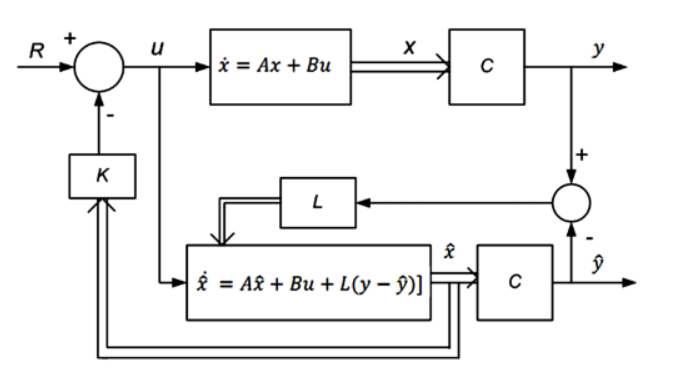
\includegraphics[width=4.5 in]{s.PNG}
  \caption{Schematic block diagram}\label{1}
\end{figure}
Finally we achieved Observer equation\\
\begin{equation}
\hat{x(k+1)} = A\hat{x(k)} + L[y(k)-\hat{y(k)}]- BK\hat{x(k)}
\end{equation}
\begin{equation}
\hat{y(k)} = C\hat{x(k)} - DK\hat{x(k)}
\end{equation}
As shown in Figure \ref{1} \cite{vinodh2013comparison}, compact form of the equations summarized as
\begin{equation}
\hat{x(k+1)} = (A- BK)\hat{x(k)} + L[y(k)-\hat{y(k)}]
\end{equation}
\begin{equation}
\hat{y(k)} = (C- DK)\hat{x(k)}
\end{equation}
Here, K and L can be selected independently to avoid any stability loss to the system.  Usually observer poles from (A-LC) are selected for rapid convergence than the state feedback poles from (A-BK).

\section*{Inference}
Lecture notes has discussed the state estimation problem in linear time invariant discrete-time-system using minimal order Luenberger State Observer. 
\bibliographystyle{ieeetran}
\bibliography{ref_observer}
\end{document}